\section{Architecture}\label{sec:architecture}

A Web application developed using the \brand{x-project} toolkit, an \brand{x-project} app, is a full stack {\em JavaScript} Single Page Application.

\paragraph{Server side}

On the server-side, an \brand{x-project} app is based on the following:

\begin{description}
\itemsep1pt\parskip0pt\parsep0pt
\item[StrongLoop LoopBack] generates model API from the models schemas, to let CRUD operations on models.
These schemas are JSON documents. Each document represents a model and presents the following fields: the \texttt{name} of the model, the set of \texttt{properties}, the list of \texttt{relations} to others models and the list of \texttt{ACL} (Access Control Layer) rules. 
The API can be extended: the developer can add remote functions to models or add hooks to existing API to add custom behavior before and/or after the API handler (to pre-process the request and/or post-process the response). 
The resulting API is RESTful, cookie free, signed by authentication token.
By default, applications have a built-in model that represents a user, with properties \texttt{username}, \texttt{email} and \texttt{password} for login and the property \texttt{role} used by the ACL module.
{\em Loopback} also introduces an indirection layer that allows to choose from almost all particular DBMS to be used.
\end{description}

\paragraph{Client side}

On the client-side, an \brand{x-project} app is based on the following:

\begin{description}
\itemsep1pt\parskip0pt\parsep0pt

\item[Web Components] are an umbrella term for four different W3C specifications \cite{w3c}:
\emph{Custom Elements} to define custom HTML elements;
\emph{HTML Templates} to define blocks of markup with the ability to inject dynamic content into;
\emph{Shadow DOM} to scope markup and styles in a separate DOM tree;
\emph{HTML Imports} to include and reuse HTML documents in other HTML documents.
Each of these pieces is useful individually. But when combined, this whole package offers:
\emph{Composability}, being able to create whole sites and apps by putting different elements together;
\emph{Encapsulation}, isolating markup, style, and behavior logic so they don't leak into the rest of the page;
\emph{Reusability}, extending existing elements to create new elements, allowing to stop reinventing the wheel.
This leads to a less fragmented ecosystem, where components can truly interoperate with each other.
Since these specifications are currently W3C Working Draft, polyfills library is required \cite{webcomponents-polyfills}.
        
\item[Polymer library] (\url{https://www.polymer-project.org/}) provides a thin layer of API on top of Web Components and several powerful features, such as custom events and delegation, mixins, accessors and component life-cycle functions, to facilitate the creation of Web Components. 
%Similar to \emph{Polymer} are \emph{x-tag} and \emph{Bosonic}. 
%Web repositories \url{http://component.kitchen} and \url{http://customelements.io} already counts thousands of open source user-contributed custom elements.
\end{description}

% \begin{figure}[!htbp]
% \centering
% 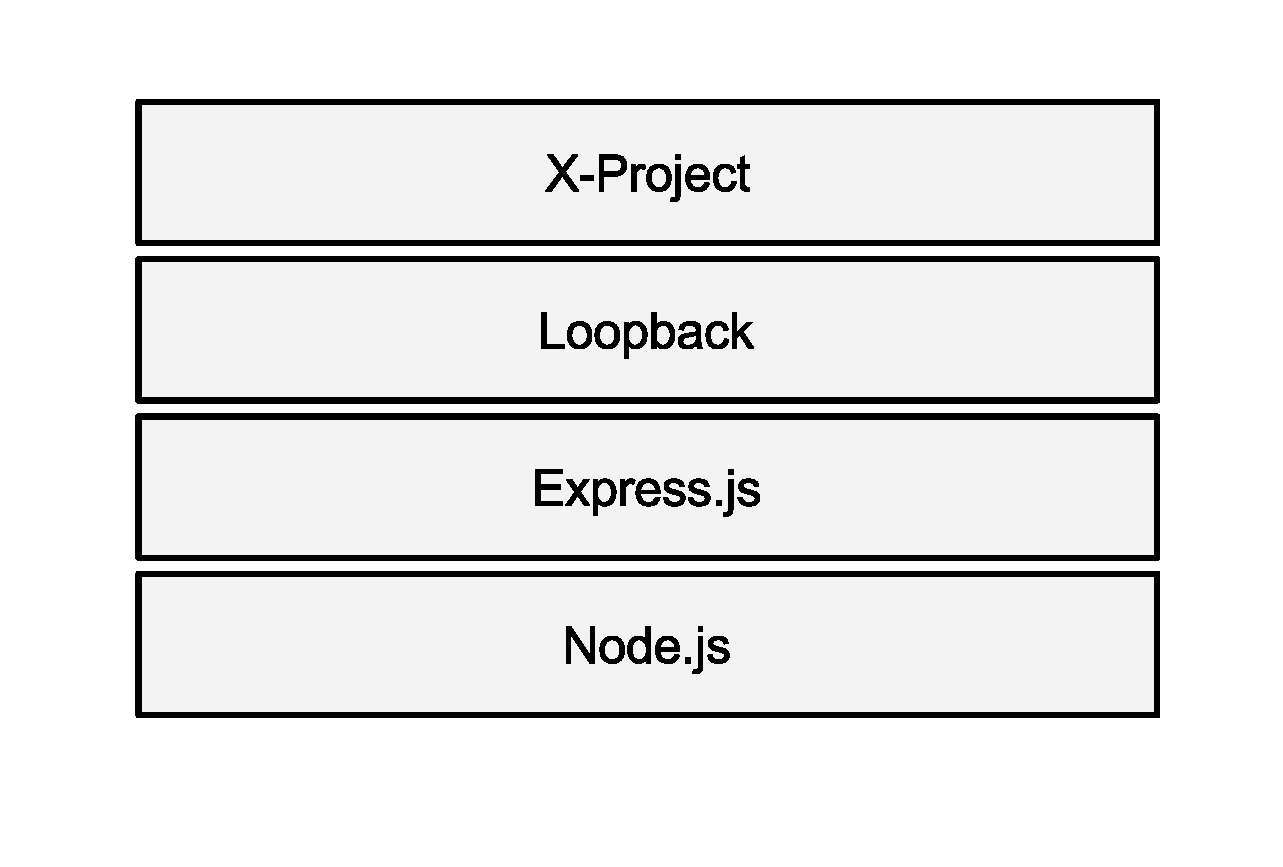
\epsfig{file=images/stack.eps, height=0.2\textwidth}
% \caption{Technology stack}
% \label{fig:tech-stack}
% \end{figure}

% \begin{figure}[!h]
%  \centering
%  \begin{subfigure}[b]{0.53\linewidth}
%  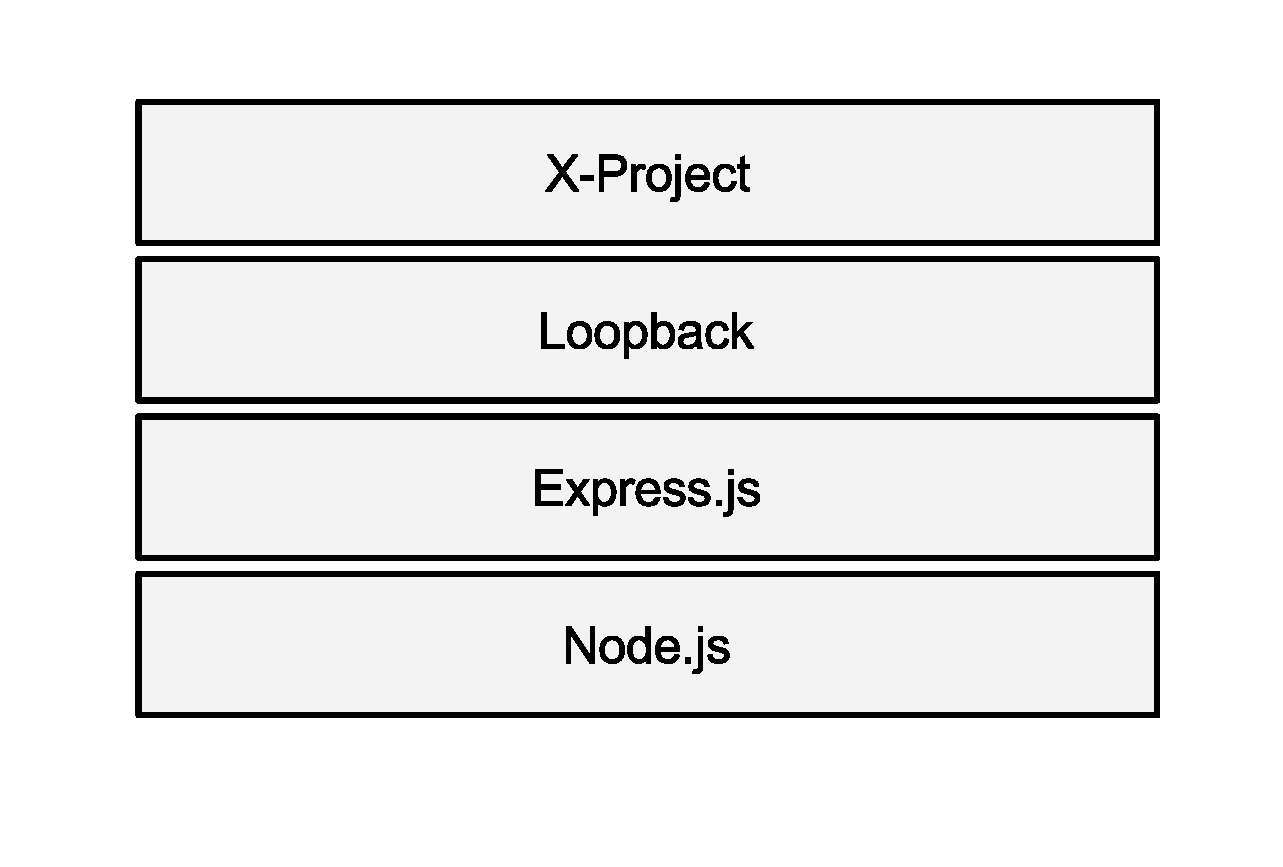
\includegraphics[width=\textwidth]{images/stack.eps} 
%  \caption{Technology stack.}
%  \label{fig:tech-stack}
%  \end{subfigure}
%  ~
%  \begin{subfigure}[b]{0.43\linewidth}
%  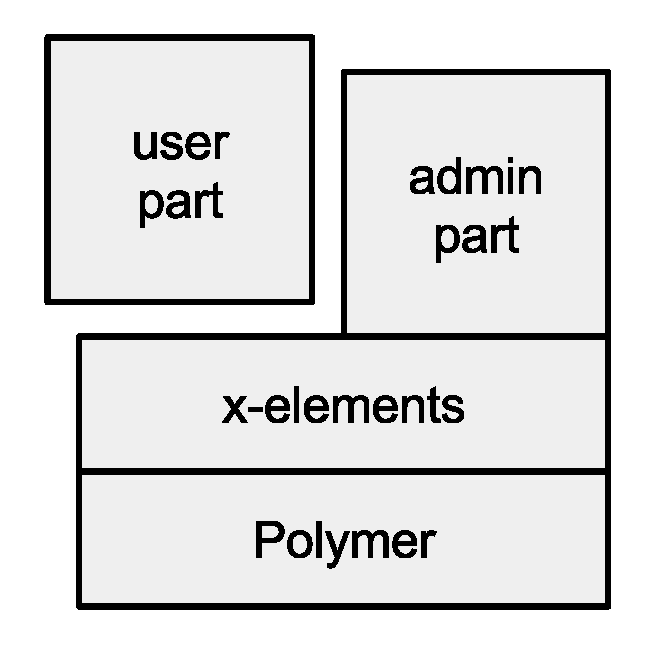
\includegraphics[width=\textwidth]{images/client-arch.eps}
%  \caption{Client-side architecture}
%  \label{fig:client-arch}
%  \end{subfigure}
 
%  % \caption{Office building: 
%  % (a) the schematic plan; 
%  % (b) the simplified 3D model generated for testing on the field 
%  % the indoor mapping project described in this paper.
%  % }
%  % \label{fig:sogei}
% \end{figure}

% \begin{figure}[!htbp]
% \centering
% 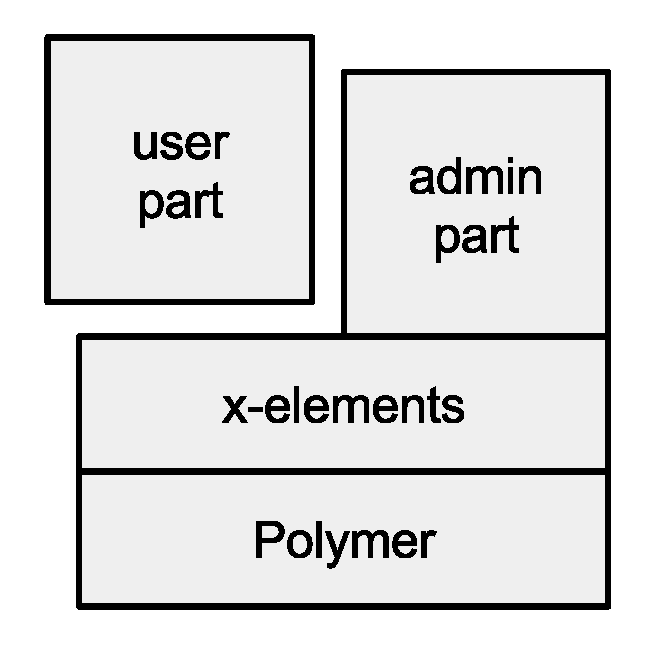
\epsfig{file=images/client-arch.eps, height=0.2\textwidth}
% \caption{Client-side architecture}
% \label{fig:client-arch}
% \end{figure}

